\documentclass[a4paper, 12pt, titlepage]{article}

\usepackage[T2A,T1]{fontenc}
\usepackage[utf8]{inputenc}
\usepackage[russian,english]{babel}
\usepackage{graphicx}
\usepackage{fullpage}
\usepackage{enumitem}
\usepackage[hidelinks]{hyperref}
\usepackage{listings}

\lstset{language=Python,
numberstyle=\footnotesize,
basicstyle=\ttfamily\tiny,
numbers=left,
stepnumber=1,
frame=shadowbox,
breaklines=true}


\begin{document}

\begin{otherlanguage}{russian}

\begin{titlepage}
\begin{center}
  
\includegraphics[scale=0.5]{label.jpg}\\
  \vspace{20pt}
  МИНОБРНАУКИ РОССИИ\\
      Федеральное государственное бюджетное образовательное учреждение\\
      высшего профессионального образования\\
    <<Московский государственный технический университет радиотехники,\\
    электроники и автоматики>>\\ 
    (МГТУ МИРЭА)\\
    \line(2,0){500}\\
    \vspace{10pt}
    {\large Факультет\\
      \vspace{10pt}
      <<Информационных технологий (ИТ)>>}
\end{center}

\vspace{60pt}
\begin{center}
  {\large Отчет}\\
  \vspace{10pt}
  О выполнении лабораторной работы №2\\
  по дисциплине <<Реляционные базы данных>>\\
\end{center}
\vspace{\fill}
Руководитель: Скворцова Л.А.\\
Исполнитель: Кулёв П.С.\\
Группа: ИТО-1-10
\begin{center}
\vspace{\fill}
Москва\\2013
\end{center}
\end{titlepage}

\newpage

\tableofcontents
\newpage

\section{Введение}
\vspace{15mm}
\par Бурное развитие информационных технологий обусловило необходимость выработки новых подходов к решению проблем автоматизации деятельности различных организаций, служб, предприятий. Работа таких организаций связана с накоплением большого количества информации.\\

\par В недавнем прошлом, информацию такого рода хранили в картотеках, используя <<бумажные>> технологии. И, разумеется, они занимали довольно большие объёмы. Вся информация заносилась вручную на бумажные карточки, что создавало большие неудобства, затрачивалось большое количество времени и, естественно, работа такого вида сама по себе была очень кропотливой. При необходимости узнать информацию требовалась затратить большое количество времени. Сама картотека <<изнашивалась>> по ходу работы, то есть через некоторое время бумага могла утратить своё былое качество.

\par Сейчас же, в век компьютерных технологий и большого прогресса в этой сфере, на смену неудобного прошлого пришли очень удобные, надёжные, быстродействующие компьютерные системы, но при этом часто возникают ситуации, когда трудно осуществить быстрый отбор нужной информации. Немаловажен вопрос надежности хранения и конфиденциальности различных сведений. Для решения таких задач используется специальное программное обеспечение, часто объединенное в крупные информационно-справочные системы.\\

\par В рамках курсовой работы ведётся разработка базы данных для учёта изготовленных в студии трехмерных цифровых моделей. Тема разработки – Разработка ПП АИС <<Модель>>.

\newpage

\section{Теоретический раздел}
\subsection{Основы разработки ПО АИС}
\vspace{15mm}

\par Автоматизированная информационная система (АИС) – это совокупность различных программно-аппаратных средств, которые предназначены для автоматизации какой-либо деятельности, связанной с передачей, хранением и обработкой различной информации.\\

\par В АИС за хранение любой информации отвечают:

\begin{center}
  \begin{enumerate}
  \item На физическом уровне:
    \begin{enumerate}[label*=\arabic*.]
    \item внешние накопители
    \item встроенные устройства памяти;
    \item дисковые массивы;
    \end{enumerate}
  \item На программном уровне:
    \begin{enumerate}[label*=\arabic*.]
    \item СУБД;
    \item Файловая система ОС;
    \item Система хранения мультимедиа;
    \end{enumerate}
  \end{enumerate}
\end{center}

\par В современной вычислительной технике ИС представляет собой целый программный комплекс, который дает возможность надежно хранить данные в памяти, выполнять преобразования информации и производить вычисления с помощью удобного и легкого интерфейса, так же называемого программным обеспечением (ПО).\\

\par Технологический процесс проектирования ПО состоит из следующих этапов:\\
\begin{enumerate}
\item Исследование и обоснование необходимости создания программного обеспечения.
\item Техническое задание, которое включает в себя назначение проекта, цель, практическое использование, требования к входным и выходным данным.
\item Эскизный проект. Он содержит глобальное проектное решение, дающее представление об устройстве и принципах работы проектируемого изделия. Этот этап иногда называется технико-экономическое обоснование.
\item Технический проект. На этом этапе определяются конфигурация технических средств, наличие устройств ввода вывода. Использование сети.
\item Рабочий проект. Включает в себя разработанное программное обеспечение и документацию по сопровождению.
\item Ввод в действие. Опытная эксплуатация, доработка, внедрение, эксплуатация.
\end{enumerate}

\newpage

\subsection{Обоснование выбора СУБД}
\vspace{15mm}

\par Для реализации решаемой задачи в курсовой работе необходимо осуществление следующих операций:\\
\begin{itemize}
\item Добавлять и удалять в базу данных записи.
\item Изменять и обновлять записи.
\item Быстро осуществлять поиск нужных записей по критериям поиска.
\item Создавать отчёты баз данных.
\itemНеобходим контроль за правильностью ввода данных.
\itemРабота с большим объёмом данных из разных таблиц и т.д. 
\end{itemize}

\par Все эти операции должны осуществляться в удобной для пользователя форме и не вызывать затруднений при работе. \\

\par Я выбрал для решения этой задачи следующие инструменты:
\begin{itemize}
\item СУБД \verb PostgreSQL ;
\item \verb Qt  \verb Designer  для создания интерфейса пользователя;
\item язык программирования \verb Python  для связи интерфейса пользователя с базой данных.

\par СУБД дают возможность пользователям осуществлять непосредственно управление данными, а программистам средства их обработки.
\end{itemize}

\par \verb PostgreSQL  это мощная объектно-реляционная система управления базами данных с открытыми исходными текстами, которая разрабатывается на протяжении более 15 лет и улучшает архитектуру, чем завоевала репутацию надежной, ингерированной и масштабируемой СУБД. Она работает на всех основных платформах, включая \verb Linux  , \verb UNIX  и \verb Windows , полностью соответствует \verb ACID , имеет полную поддержку ключей, объединений, представлений, триггеров, и хранимых процедур (на разных языках). Она включает большинство типов данных \verb SQL92  и \verb SQL99. Она также поддерживает хранение больших двоичных объектов (\verb BLOB's ), включая картинки, звук, или видео. Также эта замечательная СУБД имеет \verb API  для \verb C/C++ , \verb Java , \verb Perl , \verb Python , \verb Ruby , \verb Tcl , \verb ODBC , и некоторых других.
\newpage

\section{Раздел проектирования}
\subsection{Постановка задачи}
\vspace{15mm}

\par Существует студия, занимающаяся изготовлением трехмерных цифровых моделей на заказ. Каждый сотрудник работает в определенной программе (\verb 3ds  \verb Max , \verb ZBrush , etc.), один проект выполняется одним сотрудником. При обращении клиента работник определяет, какое ПО является наиболее подходящим для реализации конкретной задачи и трудоемкость проекта в человеко-часах. Результат может быть получен заказчиком в различном виде (финальный рендер, развертка и т.д.).\\

\par Разработка информационной системы <<Модель>> обусловлена необходимостью автоматизации ведения журнала заказов, а также быстрого и эффективного поиска информации по заданным параметрам. Данная система предназначена для внутреннего использования студией.

\begin{center}
  \textbf{Требования к проекту.}
\end{center}

\begin{itemize}
\item Вводимая информация:
  \begin{itemize}
  \item Спецификации заказа;
  \item Реквизиты заказчика;
  \end{itemize}
\item Хранимая информация:
  \begin{itemize}
  \item Список сотрудников, выполняющих заказы;
  \item Список заказчиков;
  \item Спецификации заказа;
  \end{itemize}

\item Справочники:
  \begin{itemize}
  \item Список ПО для создания модели;
  \item Список ПО для рендеринга модели;
  \item Список форм представления результата заказчику;
  \end{itemize}
  
\item Создаваемые отчёты:
  \begin{itemize}
  \item Отчет о выполненных проектах за определенный срок;
  \item Отчет о разрабатываемых проектах;
  \item Отчет о загруженности каждого сотрудника;
  \item Отчет о заказах определенного клиента;
  \item Отчет о загруженности сотрудников.
  \end{itemize}
  
\end{itemize}

\newpage

\subsection{Постановка задачи}
\subsubsection{Описание предметной области}
\vspace{10mm}

\par Представим, что в некоторой дизайнерской студии ООО <<Pafnuty\'s>> хранятся сведения о программах, в которых создаются и рендерятся проекты, о моделях, заказанных клиентами, о формах получения заказа, список заказчиков. Как  только работник определил, какое ПО является наиболее подходящим для реализации конкретной задачи, он приступает к ее выполнению. Программы создания, рендера и форма получения результата фиксируются в базе сразу же, при создании записи о новой модели. Трудоемкость вносится при завершении проекта в часах, потраченных на разработку. \\

\par Предметная область включает в себя следующие сущности:

\begin{itemize}
\item Создатель:
  \begin{itemize}
  \item ФИО
  \item Должность в фирме
  \end{itemize}
\item Модель (заказ):
  \begin{itemize}
  \item Дата открытия
  \item Дата закрытия
  \item Программа для исполнения
  \item Программа для рендера
  \item Время, затраченное на создание
  \item Форма получения
  \end{itemize}

\item Клиент:
  \begin{itemize}
  \item ФИО
  \item Адрес
  \item Контактный телефон
  \end{itemize}
\end{itemize}

\subsubsection{Проектирование концептуальной модели}
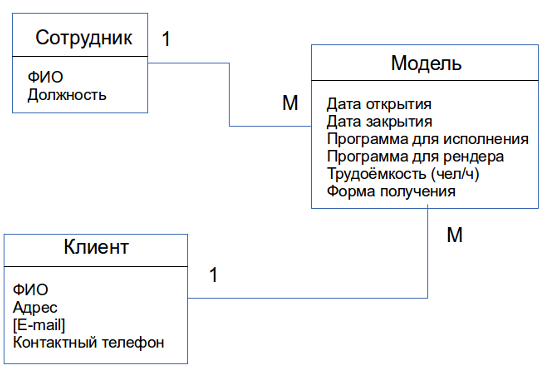
\includegraphics{concept1.png}
\subsubsection{Проектирование реляционной логической модели}
\begin{center}
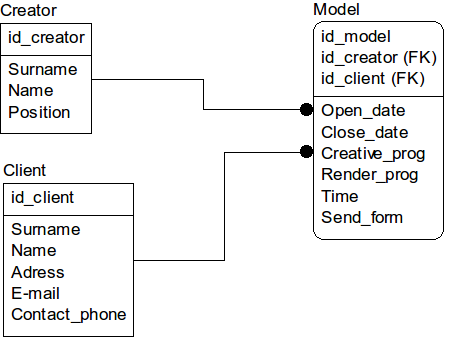
\includegraphics{relational.png}
\end{center}

\newpage
\subsubsection{Проектирование физической модели}
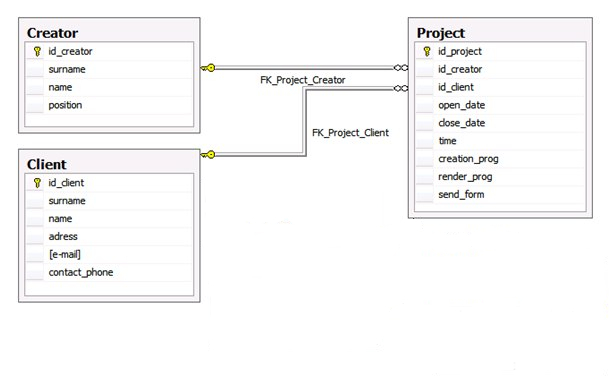
\includegraphics{erdiag.jpg}

\newpage

\section{Раздел реализации}
\vspace{30mm}
\subsection{Создание базы средствами СУБД}

\begin{enumerate}
\item Запускаем интерпретатор \verb PostgreSQL :
\begin{verbatim}
~/ $ psql -U most -d postgres 
\end{verbatim}
\item Создадим базу и подключимся к созданной базе:
\begin{verbatim}
most=# CREATE DATABASE model WITH OWNER most ENCODING 'UTF-8';
CREATE DATABASE

most=# \c model
You are now connected to database "model" as user "most".
\end{verbatim}
\item Для удобства создадим свои перечислимые типы:
{\small
\begin{verbatim}
model=# CREATE TYPE TCreationProg AS ENUM ('Blender', 'Maya', 
                                           '3ds Max', 'Houdini');
CREATE TYPE

model=# CREATE TYPE TRenderProg AS ENUM ('RenderMan', 'MentalRay', 
                                         'V-Ray', 'DreamScape');
CREATE TYPE

model=# CREATE TYPE TSendForm AS ENUM ('Model', 'Animation', 'Pictures');
CREATE TYPE

model=# CREATE TYPE TCreatorPosition AS ENUM ('Modeller', 'Animator', 
                                              '3d artist');
CREATE TYPE
\end{verbatim}}

\newpage

\item Создадим таблицы для заказчика, исполнителя и проекта:
{\small
\begin{verbatim}
model=# CREATE TABLE client (ID serial UNIQUE
model(# NOT NULL PRIMARY KEY,
model(# surname varchar(32),
model(# name varchar(32),
model(# address varchar(64),
zmodel(# email varchar(32),
model(# phone varchar(16));
NOTICE:  CREATE TABLE will create implicit sequence "client_id_seq" 
         for serial column "client.id"
NOTICE:  CREATE TABLE / PRIMARY KEY will create implicit index "client_pkey" 
         for table "client"
CREATE TABLE

model=# CREATE TABLE creator (ID serial UNIQUE
NOT NULL PRIMARY KEY,
surname varchar(32),
name varchar(32),
position TCreatorPosition);
NOTICE:  CREATE TABLE will create implicit sequence "creator_id_seq" 
         for serial column "creator.id"
NOTICE:  CREATE TABLE / PRIMARY KEY will create implicit index "creator_pkey" 
         for table "creator"
CREATE TABLE

model=# CREATE TABLE project (ID serial UNIQUE
model(# NOT NULL PRIMARY KEY,
model(# creatorID serial REFERENCES creator(ID) ON UPDATE CASCADE,
model(# clientID serial REFERENCES client(ID) ON UPDATE CASCADE,
model(# openDate date,
model(# closeDate date,
model(# time int,
model(# creationProg TCreationProg,
model(# renderProg TRenderProg,
model(# sendForm TSendForm);
NOTICE:  CREATE TABLE will create implicit sequence "project_id_seq" 
         for serial column "project.id"
NOTICE:  CREATE TABLE will create implicit sequence "project_creatorid_seq" 
         for serial column "project.creatorid"
NOTICE:  CREATE TABLE will create implicit sequence "project_clientid_seq" 
         for serial column "project.clientid"
NOTICE:  CREATE TABLE / PRIMARY KEY will create implicit index "project_pkey" 
         for table "project"
CREATE TABLE 
\end{verbatim}}

\newpage

\item Заполним таблицы тестовыми примерами:
Таблица с клиентами:
{\small
\begin{verbatim}
model=# INSERT INTO client (surname, name, address, email, phone)
model-# VALUES ('Геворкян', 'Лусинэ', 
model-#         'РФ, Сталинград г., Селезнёвой ул., 15 д., , 1 кв.', 
model(# 'louna@gmail.com', '8912334512');
INSERT 0 1

model=# INSERT INTO client (surname, name, address, email, phone)
VALUES ('Психеев', 'Фео', 'РФ, Москва г., Спартанская ул., 12 д., 5 к., 14 кв.', 
        'psiXea@gmail.com', '8991443223');
INSERT 0 1

model=# INSERT INTO client (surname, name, address, email, phone)
VALUES ('Отставников', 'Абэндон', 
        'РФ, Москва г., Нижние мневники ул., 25 д., 3\4 к., 14 кв.',   
'abandon@gmail.com', '89996663322');
INSERT 0 1
\end{verbatim}}

Заполним таблицу с сотрудниками:
{\small
\begin{verbatim}
model=# INSERT INTO creator (surname, name, position)
model-# VALUES ('Бикмамбетов', 'Тимур', '3d artist');
INSERT 0 1
model=# INSERT INTO creator (surname, name, position)
VALUES ('Миловская', 'Ольга', 'Modeller');
INSERT 0 1
model=# INSERT INTO creator (surname, name, position)
VALUES ('Порай-Кошиц', 'Пётр', 'Animator');
INSERT 0 1
\end{verbatim}}

Заполним таблицу с заказами:
{\small
\begin{verbatim}
model=# INSERT INTO project (creatorID, clientID, openDate, closeDate,
model(#                      time, creationProg, renderProg, sendForm)
model-# VALUES (1, 1, '2012-06-12', '2012-06-25',
model(#         56, 'Blender', 'RenderMan', 'Pictures');
INSERT 0 1

model=# INSERT INTO project (creatorID, clientID, openDate, closeDate,
model(#                      time, creationProg, renderProg, sendForm)
model(# VALUES (2, 2, '2012-07-21', '2012-07-25',
model(#         21, 'Maya', 'V-Ray', 'Model');
INSERT 0 1

model=# INSERT INTO project (creatorID, clientID, openDate, closeDate,
model(#                      time, creationProg, renderProg, sendForm)
model(# VALUES (3, 3, '2012-07-18', '2012-07-28',
model(#         55, 'Houdini', 'RenderMan', 'Animation');
INSERT 0 1
\end{verbatim}}

\end{enumerate}

\newpage

\subsection{Создание интерфейса пользователя}
\par Интерфейс создавался в \verb QtDesigner . Форма для авторизации в приложении сделана кодом. \\
Основная форма приложения и форма подтверждения удаления импортируются в коде.\\

\begin{center}
Форма авторизации: \\
\includegraphics[scale = 0.5]{login.png} \\
\vspace{5mm}
При ошибке можно опять попытаться ввести данные. \\
Поведение формы при несовпадении логина или пароля: \\
\includegraphics[scale = 0.5]{login_err.png} \\
\vspace{5mm}
Добавление информации в базу организовано на вкладке <<Добавить>> \\
После удачной авторизации мы попадаем на главное окно приложения: \\
\includegraphics[scale = 0.3]{add.png} \\
\vspace{5mm} 
Удаление информации из базы происходит на вкладке <<Удалить>> \\
\includegraphics[scale = 0.3]{project_del.png} \\
\vspace{5mm}
Для удаления строки таблицы пользователь должен подтвердить свой выбор. \\
Форма подтверждения удаления: \\
\includegraphics[scale = 0.3]{delete.png} \\
\vspace{5mm}
Поиск и отчёты - в соответствующей вкладке. \\
\end{center}

\newpage

\subsection{Создание клиентского приложения}

\par Клиентское приложение написано на языке программирования \verb Python .\\
Приложение полностью кроссплатформенное и может быть перенесено на любую ОС с незначительными изменениями. \\

\par Поскольку \verb Python  имеет удобные высокоуровневые типы данных и вложенность указывается отступами а не операторными скобками, код приложения получился довольно таки небольшим.

\begin{lstlisting}
#! /usr/bin/env python
# -*- coding: utf-8 -*-

import psycopg2 as ps2
import sys
from PyQt4 import QtCore, QtGui, uic

class LoginWindow(QtGui.QDialog):
    def __init__(self):
        QtGui.QDialog.__init__(self)
        self.textName = QtGui.QLineEdit(self)
        self.textPass = QtGui.QLineEdit(self)
        self.buttonLogin = QtGui.QPushButton('Login', self)
        self.buttonLogin.clicked.connect(self.handleLogin)
        layout = QtGui.QVBoxLayout(self)
        layout.addWidget(self.textName)
        layout.addWidget(self.textPass)
        layout.addWidget(self.buttonLogin)

    def handleLogin(self):
        if (self.textName.text() == 'admin' and
            self.textPass.text() == 'admin'):
            self.accept()
        else:
            QtGui.QMessageBox.warning(self, 'Error', 'Bad user or password')

class DeleteDialog(QtGui.QDialog):
    def __init__(self, what, from_what):
        QtGui.QDialog.__init__(self)
        self.msg = "Delete {w} from {f} table?".format(w = what, f = from_what)
        uic.loadUi('deldial.ui', self)
        self.label.setText(self.msg)

class MainWindow(QtGui.QMainWindow):
    def __init__(self):
        QtGui.QMainWindow.__init__(self)
        uic.loadUi('main.ui', self)

        #callbacks
        self.pb_showTable.clicked.connect(self.showTable)
        
        self.rb_client.clicked.connect(self.rb_to_pb_client)
        self.rb_creator.clicked.connect(self.rb_to_pb_creator)
        self.rb_project.clicked.connect(self.rb_to_pb_project)
        
        #add to DB callbacks
        self.pb_addClient.clicked.connect(self.addClientToDB)
        self.pb_addCreator.clicked.connect(self.addCreatorToDB)
        self.pb_addProject.clicked.connect(self.addProjectToDB)
        #remove from DB callbacks
        self.pb_delClient.clicked.connect(self.delClient)
        self.pb_delCreator.clicked.connect(self.delCreator)
        self.pb_delProject.clicked.connect(self.delProject)
        #modify callbacks
        self.pb_changeClient.clicked.connect(self.changeClient)
        self.pb_changeCreator.clicked.connect(self.changeCreator)
        self.pb_changeProject.clicked.connect(self.changeProject)

        #Database variables
        self.conn = None
        #delete if not needed
        self.cur = None
        self.data = None

    #Database features
    def connectToDB(self, db, usr):
        """db and usr are strings. If all is OK links to conn connection object"""
        try:
            self.conn = ps2.connect(database = db, user = usr)
        except ps2.DatabaseError as e:
            QtGui.QMessageBox.warning(None, 'Error', str(e))
            return False
        else:
            return True

    def disconnect(self):
        """if connection is open - closes it, otherwise prints message"""
        if self.conn.closed:
            print "Already closed"
        else:
            self.conn.close()
        
    def showTable(self):
        def getTableChoise(self):
            if self.rb_client.isChecked():
                return "client"
            elif self.rb_creator.isChecked():
                return 'creator'
            elif self.rb_project.isChecked():
                return 'project'

        def extractColumnNames(self, table):
            """table is string from which table is needed to extract names
                                         returns list of column names"""
            query = """SELECT column_name FROM information_schema.columns 
                       WHERE table_name = {t}""".format(t = repr(table))
            cur = self.conn.cursor()
            cur.execute(query)
            tupledList = cur.fetchall()
            resList = []
            for i in tupledList:
                resList.append(i[0])
            resList.reverse()
            return resList
        
        def replaceIDs(self, cur_table):
#            query = """SELECT idj from 
            pass

        #connect to DB and get table and column labels
        self.connectToDB('model', 'most')
        cur = self.conn.cursor()
        cur_what = '*'
        cur_table = getTableChoise(self)
        query = 'SELECT {what} FROM {table};'.format(what = cur_what, table = cur_table)
        cur.execute(query)
        data = cur.fetchall()
        names = extractColumnNames(self, cur_table)
        self.disconnect()

        lines = len(data)
        columns = len(data[0])
        self.tableWidget.setSortingEnabled(True)
        self.tableWidget.setRowCount(lines)
        self.tableWidget.setColumnCount(columns)

        self.tableWidget.setHorizontalHeaderLabels(names)
        for i in xrange(lines):
            for j in xrange(columns):
                decoded = data[i][j]
                decoded = str(decoded).decode('utf-8')    
                item = QtGui.QTableWidgetItem(decoded)
                self.tableWidget.setItem(i, j, item)
        self.tableWidget.sortByColumn(0, QtCore.Qt.AscendingOrder)

    #radiobuttons features
    def rb_to_pb_client(self):
        self.pb_showTable.setText('Show client table')
    def rb_to_pb_creator(self):
        self.pb_showTable.setText('Show creator table')
    def rb_to_pb_project(self):
        self.pb_showTable.setText('Show project table')

    
    def addClientToDB(self):
        class Client:
            pass

        Client.Surname = str(self.le_clientSurname.text())
        Client.Name = str(self.le_clientName.text())
        Client.Address = str(self.le_clientAddress.text())
        Client.Email = str(self.le_clientEmail.text())
        Client.Phone = str(self.le_clientPhone.text())
        if (Client.Surname == "" or Client.Name == "" or Client.Address == ""
            or Client.Email == "" or Client.Phone == ""):
            QtGui.QMessageBox.warning(self, 'Error', 'One or more fields are empty!')
        else:
            query = """INSERT INTO client (surname, name, address, email, phone)
                       VALUES ({s}, {n}, {a}, {e}, {p});
                    """.format(s = repr(Client.Surname), n = repr(Client.Name), 
                               a = repr(Client.Address), e = repr(Client.Email), 
                               p = repr(Client.Phone))
            try:
                self.connectToDB('model', 'most')
                cur = self.conn.cursor()
                cur.execute(query)
                self.conn.commit()
    
            except ps2.DatabaseError as e:
                if self.conn:
                    self.conn.rollback()
                    QtGui.QMessageBox.warning(self, 'Error', str(e))
            finally:
                self.disconnect()
                
    def addCreatorToDB(self):
        class Creator:
            pass
        
        Creator.Surname = unicode(self.le_creatorSurname.text()).encode('utf-8')
        Creator.Name = str(self.le_creatorName.text())
        Creator.Position = str(self.cb_creatorPosition.currentText())
        print Creator.Surname
        if (Creator.Surname == "" or Creator.Name == ""):
            QtGui.QMessageBox.warning(self, 'Error', 'One or more fields are empty!')
        else:
            query = """INSERT INTO creator (surname, name, position)
                       VALUES ({s}, {n}, {p});
                    """.format(s = repr(Creator.Surname), n = repr(Creator.Name), 
                               p = repr(Creator.Position))
            try:
                self.connectToDB('model', 'most')
                cur = self.conn.cursor()
                cur.execute(query)
                self.conn.commit()
            except ps2.DatabaseError as e:
                if self.conn:
                    self.conn.rollback()
                    QtGui.QMessageBox.warning(self, 'Error', str(e))
            finally:
                self.disconnect()

    def addProjectToDB(self):
        def parseDate(original):
            date = original[(original.index("(") + 1) : original.index(")")]
            digits = [str(i) for i in range(10)]
            result = ""
            for char in date:
                if char == ',':
                    result += '-'
                elif char in digits:
                    result += char
                else:
                    pass
                
            return result

        class Project:
            pass

        Project.CreatorID = str(self.le_projectCreatorID.text())
        Project.ClientID = str(self.le_projectClientID.text())
        Project.OpenDate = parseDate(str(self.de_projectOpenDate.date()))
        Project.CloseDate = parseDate(str(self.de_projectCloseDate.date()))
        Project.Time = str(self.sb_projectTime.text())
        Project.CreationProg = str(self.cb_projectCreationProg.currentText())
        Project.RenderProg = str(self.cb_projectRenderProg.currentText())
        Project.SendForm = str(self.cb_projectSendForm.currentText())
        if (Project.CreatorID == "" or Project.ClientID == "" or Project.Time == ""):
            QtGui.QMessageBox.warning(self, 'Error', 'One or more fields are empty!')
        else:
            query = """INSERT INTO project (creatorID, clientID, openDate, closeDate,
                                            time, creationProg, renderProg, sendForm)
                       VALUES ({creator}, {client}, {od}, {cd}, {t}, {cp}, {rp}, {sf});
                    """.format(creator = repr(Project.CreatorID), 
                               client = repr(Project.ClientID), 
                               od = repr(Project.OpenDate), 
                               cd = repr(Project.CloseDate), 
                               t = Project.Time,     #without repr because in DB - int
                               cp = repr(Project.CreationProg),
                               rp = repr(Project.RenderProg),
                               sf = repr(Project.SendForm))
            
            try:
                self.connectToDB('model', 'most')
                cur = self.conn.cursor()
                cur.execute(query)
                self.conn.commit()
            except ps2.DatabaseError as e:
                if self.conn:
                    self.conn.rollback()
                    QtGui.QMessageBox.warning(self, 'Error', str(e))
            finally:
                self.disconnect()

    def abstractDel(self, table, object_id = None, surname = None, name = None):
        if surname == None and name == None and object_id:
            query = """DELETE FROM {t} WHERE id = {i}""".format(t = table, 
                                                                i = object_id)
        elif surname and name and object_id == None:
            query = """DELETE FROM {t} WHERE surname = {s} 
                                             AND name = {n}""".format(t = table, 
                                                                      s = repr(surname),
                                                                      n = repr(name))
        else:
            QtGui.QMessageBox(self, 'Error', 'One field is empty')
            return

        try:
            self.connectToDB('model', 'most')
            cur = self.conn.cursor()
            cur.execute(query)
            self.conn.commit()
        except ps2.DatabaseError as e:
            if self.conn:
                QtGui.QMessageBox(self, 'Error', str(e))
                self.conn.rollback()
        finally:
            self.disconnect()


    def delClient(self):
        #get info
        
        if self.rb_delClientByID.isChecked():
            clientID = str(self.le_delClientID.text())
            clientSurname = None
            clientName = None
        else:
            clientSurname = str(self.le_delClientSurname.text())
            clientName = str(self.le_delClientName.text())
            clientID = None

        #set parameters
        w = DeleteDialog('this record', 'client')
        if w.exec_() == QtGui.QDialog.Accepted:
            self.abstractDel('client', clientID, clientSurname, clientName)
            self.showTable()
    
    def delCreator(self):
        #get info
        if self.rb_delCreatorByID.isChecked():
            creatorID = str(self.le_delCreatorID.text())
            creatorSurname = None
            creatorName = None
        else:
            creatorSurname = str(self.le_delCreatorSurname.text())
            creatorName = str(self.le_delCreatorName.text())
            creatorID = None

        #set parameters
        w = DeleteDialog('this record', 'creator')
        if w.exec_() == QtGui.QDialog.Accepted:
            self.abstractDel('creator', creatorID, creatorSurname, creatorName)
            self.showTable()

    
    def delProject(self):
        projectID = str(self.le_delProjectID.text())

        w = DeleteDialog('this record', 'project')
        if w.exec_() == QtGui.QDialog.Accepted:
            self.abstractDel('project', object_id = projectID)
            self.showTable()

    def abstractChange(self, table, field, target, ident):
        query = "UPDATE {T} SET {f} = {t} WHERE id = {i}".format(
            T = table,
            f = field,
            t = repr(target),
            i = ident)
        try:
            self.connectToDB('model', 'most')
            cur = self.conn.cursor()
            cur.execute(query)
            self.conn.commit()
        except ps2.DatabaseError as e:
            QtGui.QMessageBox.warning(self, 'Error', str(e))
            if self.conn:
                self.conn.rollback()
        finally:
            self.conn.close
        
    def changeClient(self):
        table = 'client'
        ident = str(self.le_changeClientID.text())
        field = str(self.cb_changeClientField.currentItem())
        target = str(self.le_changeClientTarget.text())
        self.abstractChange(table, field, target, ident)
        self.rb_client.setEnabled(True)
        self.showTable()

    def changeCreator(self):
        table = 'creator'
        ident = str(self.le_changeCreatorID.text())
        field = str(self.cb_changeCreatorField.currentText())
        target = str(self.le_changeCreatorTarget.text())
        self.abstractChange(table, field, target, ident)
        self.rb_creator.setEnabled(True)
        self.showTable()

    def changeProject(self):
        table = 'project'
        ident = str(self.le_changeProjectID.text())
        field = str(self.cb_changeProjectField.currentText())
        target = str(self.le_changeProjectTarget.text())
        self.abstractChange(table, field, target, ident)
        self.rb_project.setEnabled(True)
        self.showTable()



def login(login):
    l = login()    
    return l.exec_() == QtGui.QDialog.Accepted


if __name__ == '__main__':
    app = QtGui.QApplication(sys.argv)
    if login(LoginWindow):
        w = MainWindow()
        w.show()
        sys.exit(app.exec_())
\end{lstlisting}

\newpage

\section{Заключение}
\par В ходе работы в соответствии с поставленной задачей была разработана база данных <<Модель>>. Для этого была описана предметная область, спроектированы и реализованы ее концептуальная модель, реляционная логическая модель, физическая модель базы данных.
\section{Библиографический список}

\begin{enumerate}
\item Голицына О. Л., Максимов Н. В., Попов И. И. Базы данных: учеб. Пособие. – 2-е изд., испр. И доп. – М.: ФОРУМ: ИНФРА-М, 2007. 
\item \url{http://www.postgresql.org}
\item \url{http://www.python.org}
\item \url{http://stackoverflow.com}
\end{enumerate}


\end{otherlanguage}
\end{document}
